\section{Headline evaluation: corpus replication}
\label{sec:corpus}

\paragraph{Question.} Given only a person's name and birth year, how much of a hand-built genealogical dossier can each strategy recover in one pass? This is the evaluation the author cares about most: the dossiers took weeks of supervised work, and the point of \CR is to do that work without the supervisor. It was designed after the preregistration (\cref{sec:bench}); we report it as the headline because it scores the task end to end, and we keep the preregistered record-level results (\cref{sec:results}) separate.

\paragraph{Gold set.} Six deceased people with dossiers from the author's own family research, chosen for different kinds of life: a Civil War soldier (Erastus W.\ Burnham, 1834 to 1921), a World War~I veteran (Homer D.\ St.\ John, 1900 to 1972), a World War~II veteran (John St.\ John, 1921 to 2006) and three civilians (Kingsley A.\ Perry, 1907 to 1962; Edgar H.\ Bristol, 1871 to 1944; Alex St.\ John, 1967 to 2026). Five have a death in their own dossier; Alex's gate basis is the author's attestation of 26 November 2026. A model split each dossier into atomic facts, each with its sources and an access tier (open web, gated web, book, outreach); the keys are frozen and hash-locked as answer key \RESULT{corpus-key}. Facts about living relatives are withheld from the public key.

\paragraph{Protocol.} Every strategy gets the same input (name and birth year), the same keyless tools (Internet Archive catalogue, full text and search inside a book; Chronicling America; Wikidata), the same budget of 100 tool calls, and \RESULT{corpus-runs} runs per person. An exclusion filter at the tool layer blocks the author's own websites, repositories, deployments and accounts and archive snapshots of them, and drops any returned page whose word 8-grams overlap the dossier text; it was on for every run (\cref{tab:leak}). A fact earns 1.0 when it is found in the evidence the tools returned, near a mention of the right person, with its year when it has one; 0.5 when the strategy reached the fact's source record or named the right book or archive; 0 otherwise.

\begin{table*}[t]\centering\small
\resizebox{\textwidth}{!}{\begin{tabular}{@{}lcccccccccc@{}}
\toprule
Strategy & Burnham (Civil War) & Homer (WWI) & John (WWII) & Kingsley (civilian) & Bristol (civilian) & Alex (civilian) & Overall & Reachable & Precision & Penalised \\
\midrule
B0 single-pass LLM search & 13.7$\pm$0.4 & 0.0$\pm$0.0 & 0.0$\pm$0.0 & 6.5$\pm$2.7 & 19.2$\pm$15.6 & 2.1$\pm$0.0 & 6.9\% & 14.3\% & 30.5\% & 6.9\% \\
B1 ReAct LLM agent & 18.6$\pm$1.0 & 0.0$\pm$0.0 & 0.0$\pm$0.0 & 8.5$\pm$1.1 & 35.8$\pm$0.7 & 6.4$\pm$2.0 & 11.6\% & 22.0\% & 49.3\% & 11.3\% \\
B3 checklist only & 0.0$\pm$0.0 & 0.0$\pm$0.0 & 0.0$\pm$0.0 & 0.0$\pm$0.0 & 0.0$\pm$0.0 & 2.1$\pm$0.0 & 0.4\% & 1.1\% & 57.4\% & 0.4\% \\
B5 CR (preregistered) & 17.5$\pm$0.0 & 0.0$\pm$0.0 & 0.0$\pm$0.0 & 1.9$\pm$0.0 & 35.6$\pm$0.0 & 3.9$\pm$0.9 & 9.8\% & 19.4\% & 66.9\% & 9.5\% \\
B5-max CR wider (post hoc) & 18.1$\pm$0.0 & 0.0$\pm$0.0 & 0.0$\pm$0.0 & 1.9$\pm$0.0 & 36.2$\pm$0.0 & 3.9$\pm$0.9 & 10.0\% & 19.7\% & 65.7\% & 9.7\% \\
B5-fix CR rules2 (post hoc fix) & 22.6$\pm$0.0 & 0.0$\pm$0.0 & 0.0$\pm$0.0 & 11.4$\pm$0.0 & 36.2$\pm$0.0 & 3.9$\pm$0.9 & 12.4\% & 24.4\% & 67.2\% & 11.6\% \\
B5-llm CR, model question generator (ablation, post hoc) & 14.1$\pm$1.0 & 0.0$\pm$0.0 & 0.0$\pm$0.0 & 5.2$\pm$4.2 & 31.4$\pm$3.8 & 4.9$\pm$0.0 & 9.3\% & 18.8\% & 32.0\% & 9.1\% \\
\bottomrule
\end{tabular}}
\caption{Corpus replication (answer key v1): percent of each hand-built dossier recovered in one pass, mean$\pm$sd over runs. 1.0 per fact found in returned evidence, 0.5 for reaching the right record or naming the right book or archive, 0 otherwise. Reachable: mean recall on facts with a source on a host the tools query (Homer has none). Precision: share of cited items that name the subject inside his life span. Penalised subtracts 5 per false family link per fact. Generated by \texttt{eval/fill\_v0.py} from \texttt{benchmark/results}.}
\label{tab:corpus}
\end{table*}


\paragraph{Result.} The preregistered \CR configuration (B5) recovered \RESULT{corpus-overall-B5} of the six dossiers on average, against \RESULT{corpus-overall-B1} for a ReAct agent (B1) and \RESULT{corpus-overall-B0} for single-pass search (B0); the checklist alone (B3) recovered \RESULT{corpus-overall-B3}. \textbf{CR lost to ReAct}: it was behind on \RESULT{corpus-B5-vs-B1-wl} (mean difference \RESULT{corpus-B5-vs-B1-diff} points, exact sign-flip $p=$\,\RESULT{corpus-B5-vs-B1-p}). It beat single pass (\RESULT{corpus-B5-vs-B0-wl}). The best CR variant, B5-fix, a post hoc repair of the rule generator described below, recovered \RESULT{corpus-overall-B5fix} (\RESULT{corpus-B5fix-vs-B1-wl} against B1, $p=$\,\RESULT{corpus-B5fix-vs-B1-p}). With six people no difference reaches significance; the smallest possible two-sided $p$ is 0.031, and after Holm correction every comparison is above 0.8. CR was the most precise strategy: \RESULT{corpus-prec-B5} of the items it cited named the subject inside his life span, against \RESULT{corpus-prec-B1} for B1 and \RESULT{corpus-prec-B0} for B0. It also made the most false family links (\RESULT{corpus-fl-B5} for B5 and \RESULT{corpus-fl-B5fix} for B5-fix over all runs, against \RESULT{corpus-fl-B1} for B1), CR's links all came from one passage that names Burnham's grandparents as his parents (\cref{sec:wrongparents}); B1's came from a Homer run.

\begin{table}[t]\centering\small
\resizebox{\columnwidth}{!}{\begin{tabular}{@{}lccccccc@{}}
\toprule
& Burnham & Homer & John & Kingsley & Bristol & Alex & Mean \\
Reachable facts & 111/226 & 0/109 & 2/102 & 144/232 & 61/87 & 89/233 & \\
\midrule
B0 & 27.9 & \NM & 0.0 & 10.5 & 27.3 & 5.6 & 14.3\% \\
B1 & 33.9 & \NM & 0.0 & 11.2 & 51.1 & 13.7 & 22.0\% \\
B3 & 0.0 & \NM & 0.0 & 0.0 & 0.0 & 5.6 & 1.1\% \\
B5 & 32.9 & \NM & 0.0 & 3.1 & 50.8 & 10.3 & 19.4\% \\
B5-max & 33.3 & \NM & 0.0 & 3.1 & 51.6 & 10.3 & 19.7\% \\
B5-fix & 41.4 & \NM & 0.0 & 18.4 & 51.6 & 10.3 & 24.4\% \\
B5-llm & 27.8 & \NM & 0.0 & 8.3 & 44.8 & 12.9 & 18.8\% \\
\bottomrule
\end{tabular}}
\caption{The reachability ceiling. A fact is reachable when one of its dossier sources is on archive.org, loc.gov or wikidata.org, the only hosts the bench tools query. Recall (\%) on the reachable facts only; Homer has no reachable fact (\NM). Generated from results.}
\label{tab:reach}
\end{table}


\begin{figure*}[t]\centering
\IfFileExists{figures/corpus-recall.pdf}{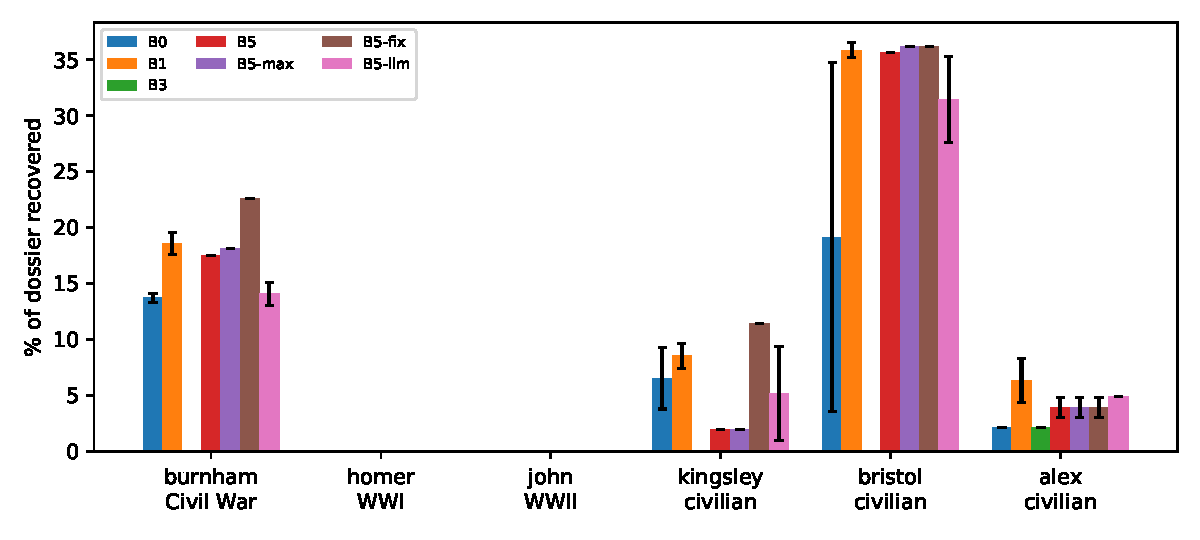
\includegraphics[width=0.92\textwidth]{figures/corpus-recall.pdf}}{\NM}
\caption{Share of each dossier recovered, per person and strategy, mean and sd over runs. Generated by \texttt{eval/corpus/report.py}.}
\label{fig:corpus}
\end{figure*}

\paragraph{The reachability ceiling is the larger finding.} Most dossier facts came from sources these tools cannot reach. Only \RESULT{corpus-reachn-homer} of Homer's facts and \RESULT{corpus-reachn-john} of John's have a source on archive.org, loc.gov or wikidata.org; their dossiers rest on obituaries in paywalled newspaper archives, military records behind logins, and family interviews. Every strategy scored zero on both. Scored on the reachable facts only (\cref{tab:reach}), B5 recovered \RESULT{corpus-reach-B5}, B1 \RESULT{corpus-reach-B1}, B0 \RESULT{corpus-reach-B0} and B5-fix \RESULT{corpus-reach-B5fix}. The ranking does not change, but the absolute numbers say that tool access, not question generation, sets the ceiling on this task.

\paragraph{Why CR underperformed (post hoc diagnosis).} We read the tool logs of every run (\cref{tab:diagnose}). Six causes stand out.
\begin{enumerate}
\item \emph{It stops early.} The preregistered B5 used \RESULT{diag-calls-B5} tool calls per run of its 100; its rule generator ran out of new questions. B1 used \RESULT{diag-calls-B1}.
\item \emph{It repeats itself.} \RESULT{diag-repeat-B5} of B5's calls, and \RESULT{diag-repeat-B5max} of B5-max's, were exact repeats of an earlier call in the same run, mostly the same search inside the same book asked again from different branches of the graph. ReAct repeated \RESULT{diag-repeat-B1}.
\item \emph{The checklist assumes a birthplace.} With only a name and a year, the checklist built empty queries (a title search for a town it did not have) and searched the full name with its middle name only; B3 scored zero for five of six people and \RESULT{diag-empty-B3} of its calls came back empty.
\item \emph{Name forms.} The rule generator parsed ``Homer Doble St.\ John'' with the surname ``John'' and never tried ``H.\ D.\ St.\ John'' or ``Homer D.\ St.\ John'', the forms the records use.
\item \emph{Namesakes.} Its searches pulled in the father and the son who share Burnham's name, and one passage about the father produced the wrong-parents link.
\item \emph{A model generator did not help here.} CR with a model writing its questions (B5-llm) recovered \RESULT{corpus-overall-B5llm}, below the rule generator, and the items it cited were less often about the subject (precision \RESULT{corpus-prec-B5llm}). On the record-level benchmark the same generator was the best CR variant (\cref{tab:ablate}), so the evidence on model-written questions is mixed.
\end{enumerate}
B5-fix repairs the second, fourth and part of the first cause (a ``St.''\ surname particle rule, name forms, de-duplication of planned calls, and continuing until the budget or the leads run out). It lifted CR from \RESULT{corpus-overall-B5} to \RESULT{corpus-overall-B5fix}, but it was tuned while looking at Burnham, so it is post hoc and its edge over B1 is not a test.

\begin{table*}[t]\centering\small
\begin{tabular}{@{}lcccccccc@{}}
\toprule
Strategy & Calls/run & Exact repeats & Empty results & Items returned & On target & IA full text & Inside a book & Newspapers \\
\midrule
B0 & 7.4 & 0.0\% & 50.2\% & 21 & 33.1\% & 2.1 & 0.0 & 2.2 \\
B1 & 22.4 & 0.6\% & 49.5\% & 466 & 22.7\% & 5.3 & 4.8 & 4.9 \\
B3 & 7.2 & 30.4\% & 75.6\% & 7 & 22.8\% & 0.0 & 0.0 & 1.2 \\
B5 & 17.0 & 41.4\% & 48.5\% & 537 & 42.2\% & 2.5 & 4.0 & 3.5 \\
B5-max & 41.8 & 52.7\% & 37.7\% & 1413 & 32.3\% & 2.8 & 24.1 & 6.3 \\
B5-fix & 46.4 & 11.1\% & 39.8\% & 1105 & 15.1\% & 3.8 & 23.0 & 10.4 \\
B5-llm & 42.3 & 26.3\% & 50.3\% & 121 & 49.4\% & 18.9 & 1.2 & 13.4 \\
\bottomrule
\end{tabular}
\caption{Tool-use profile per run on the corpus, from the tool-layer logs (\texttt{eval/corpus/diagnose.py}). Exact repeats: calls identical to an earlier call in the same run. On target: share of returned items that name the subject and carry no year outside his life. The last three columns are calls per run to each tool.}
\label{tab:diagnose}
\end{table*}


\paragraph{Scorer audit.} The scorer is automatic, so we audited it. A model judge at temperature 0 saw \RESULT{corpus-audit-n} sampled decisions, half credited and half not, with the exact text window the scorer matched. It agreed with the scorer on \RESULT{corpus-audit-agree} (Cohen's $\kappa=$\,\RESULT{corpus-audit-kappa}) and confirmed \RESULT{corpus-audit-prec} of credited facts. An AI research assistant then read every disagreement against the matched text (a second reading, not a human rating): \RESULT{corpus-hand-summary}. The first audit, on scorer version 1.0, found six bugs that inflated scores, among them an 1864 Homer D.\ St.\ John counting as the World War~I veteran, Burnham's father counting as Burnham, and loc.gov URLs that echo the agent's own query. We fixed them (scorer v1.1) and report v1.1 throughout; under v1.0 every overall score was higher or equal and the ranking was the same. Read the absolute numbers as upper bounds: about one credited fact in five is not supported by its evidence.

\paragraph{Leakage.} No call reached a blocked host (\cref{tab:leak}). The content guard dropped \RESULT{corpus-dropped-B1} items for B1, \RESULT{corpus-dropped-B5max} for B5-max, \RESULT{corpus-dropped-B5fix} for B5-fix and \RESULT{corpus-dropped-B5llm} for B5-llm; we read them, and every one was a page of a primary source that the dossiers quote at length (the 1884 Burnham genealogy and catalogue records of a book about Alex St.\ John), not a copy of the author's work. The guard is therefore conservative: it cost the strategies a little recall, evenly.

\begin{table}[t]\centering\small
\begin{tabular}{@{}lccc@{}}\toprule
Strategy & Runs & Host blocks & Overlap drops \\\midrule
B0 & 18 & \RESULT{corpus-blocked-B0} & \RESULT{corpus-dropped-B0} \\
B1 & 18 & \RESULT{corpus-blocked-B1} & \RESULT{corpus-dropped-B1} \\
B3 & 18 & \RESULT{corpus-blocked-B3} & \RESULT{corpus-dropped-B3} \\
B5 & 18 & \RESULT{corpus-blocked-B5} & \RESULT{corpus-dropped-B5} \\
B5-max & 18 & \RESULT{corpus-blocked-B5max} & \RESULT{corpus-dropped-B5max} \\
B5-fix & 18 & \RESULT{corpus-blocked-B5fix} & \RESULT{corpus-dropped-B5fix} \\
B5-llm & 18 & \RESULT{corpus-blocked-B5llm} & \RESULT{corpus-dropped-B5llm} \\\bottomrule
\end{tabular}
\caption{Leakage audit: tool calls blocked by the host rule and returned items dropped by the dossier 8-gram guard, all runs.}
\label{tab:leak}
\end{table}
